%\AtBeginDvi{\special{pdf:mapfile texfonts.map}}
\documentclass[10pt]{jsarticle}
\usepackage{listings,jlisting}
\usepackage{color}
\usepackage{amsmath,amssymb}
\usepackage[dvipdfmx]{graphicx}
\usepackage{here}
\makeatletter
\def\lst@title@dropdelim\hskip1zw{}
\makeatother

%listingsの設定%{{{
\lstset{
    basicstyle = \small\ttfamily,    %ソースコードの書籍
    numbers = left,     %行番号
    numberstyle = \tiny,
    frame = {tblrTB},   %ソースコードを囲むフレーム(大文字があるところは二重線になる)
    backgroundcolor = {\color[gray]{.95}},  %数字を小さくすると黒くなる
    keywordstyle = {\small\bfseries \color[rgb]{0,0.4,0.4}},
    commentstyle = {\small\bfseries \color[rgb]{0.5,0.5,0.5}},
    identifierstyle={\small},%
    ndkeywordstyle={\small},%
    stringstyle={\small\ttfamily},
    columns=[l]{fullflexible},%
    keepspaces=true,
    showstringspaces=false,
    lineskip=-0.5zw,
}%}}}


\begin{document}
\begin{titlepage}
\title{情報実験第4 コンパイラ 課題1}
\date{\today}
\author{池田 光 \\ 学籍番号:14\_0095 \\ ログイン名:j40095 \\ メールアドレス:ikeda.h.am@m.titech.ac.jp}
\maketitle
\thispagestyle{empty}
\end{titlepage}


\section{目的}
以下をコンパイルできるように,コンパイラを拡張する.
\begin{enumerate}
\item int型の大域変数
\item 代入式(=式)
\item while文
\item $<$式
\item +式
\item -式
\end{enumerate}
これらを実装することで,簡単な計算を行うプログラムの実行が可能になるとともに,繰り返し処理をするプログラムの実行ができるようになる.
\section{変更点}
変更はすべてcodegen.cファイルにて行った.

\subsection{共通の変更点}
\subsubsection{関数の宣言について}
codegen\_global関数では,codegen\_fnction\_definition関数が呼ばれ,この関数内ではスタックフレームを作成するアセンブリコードを生成した後,構文木の各ノードの属性にあったアセンブリコードを生成するため,各ノードの属性による条件分岐を行いアセンブリコードを生成する関数を呼ぶvisit\_AST関数が呼ばれる.
そのため,本課題において,visit\_AST関数内に代入式,while文,$<$式,+式,-式のアセンブリコードを生成するための条件分岐及び関数を加えるとともに,プログラムの先頭に新たに追加した関数の定義をおこなう.これにより,各ノードの属性に対応したアセンブリコードを出力する関数をvisit\_AST関数内で呼び出しが可能となる.\\
以下に変更箇所のコードを示す.

\begin{lstlisting}[caption=visit\_AST関数内,label=visit_AST]
else if (!strcmp (ast->ast_type, "AST_statement_while")) { //while文
  codegen_statement_while (ast);
} else if (!strcmp (ast->ast_type, "AST_expression_assign")) { //代入文(=)
  codegen_expression_assign (ast);
} else if (!strcmp (ast->ast_type, "AST_expression_less")) { // <式
  codegen_expression_less (ast);
} else if (!strcmp (ast->ast_type, "AST_expression_add")) { // +式
  codegen_expression_add (ast);
} else if (!strcmp (ast->ast_type, "AST_expression_sub")) { // -式
  codegen_expression_sub (ast);
}
\end{lstlisting}

\begin{lstlisting}[caption=関数の宣言,label=関数の宣言]
static void codegen_statement_while(struct AST *ast);  //while文用関数の宣言
static void codegen_expression_assign(struct AST *ast); //代入文(=)用関数の宣言
static void codegen_expression_less(struct AST *ast);   //<式用関数の宣言
static void codegen_expression_add(struct AST *ast);    //+式用関数の宣言
static void codegen_expression_sub(struct AST *ast);    //-式用関数の宣言
\end{lstlisting}


\subsubsection{スタックフレームについて}
Mac OS Xのバイナリ形式は関数呼び出しの際,スタックポインタが16バイト境界を指すよう要求しているため,関数呼び出し時に16バイト境界を指すようにpaddingをいれる必要がある.本実験では,codegen\_expression\_funcall関数内におけるpaddingの計算において大域変数frame\_heightを用いて計算をおこなっている.そのため,各関数内においてスタックから値を取り出したとき(popを行ったとき)はframe\_heighから4を減算し,スタックへ値を積んだとき(pushを行うとき)はframe\_heightに4を加算する.

\subsection{int型の大域変数の実装}
codegen\_global関数で変更を行った.この関数はglobalな関数の宣言を行っている関数で,変更前は構文木のなかのglobal関数しかアセンブリ
コードを生成しなかったので,この中に,大域変数の宣言の記述を加えることで,大域変数についてもアセンブリコードを生成出来るようにした.
具体的な方法については,global関数の宣言と同様に,記号表から,属性がTYPE\_KIND\_PRIMであるものに関して大域変数と処理し,その変数名を
取得し,
\begin{center}
.comm \_変数名,4,2
\end{center}
にて宣言をした.本課題では,大域変数はint型なので,4バイト確保する.
以下にコードを示す.

\begin{lstlisting}[caption=大域変数の宣言,label=大域変数]
sym = sym_table.global;
while (sym != NULL) {
  if (sym->type->kind == TYPE_KIND_PRIM) {
    emit_code(sym->ast,"\t.comm\t_%s,4,2\n",sym->name);
  };
  sym = sym->next;
}
\end{lstlisting}

\subsection{代入式(=)について}
代入文のアセンブリコードの生成はcodegen\_expression\_assign関数にて行う.\\
はじめに,代入文の全体の流れを示す.右辺値の値をスタックにつみ,左辺値つまり代入先のアドレスをスタックに積む.代入先のアドレスを\%eaxに代入し,スタックトップの値を\%ecxに代入した後,\%ecxの値を\%eaxに代入する.ここで,右辺値とは右辺式を処理した返り値であることで,右辺式が計算式や代入式の場合も左辺値に代入することを可能にしている.\\
右辺値の値からスタックに積む必要があるので,子ノードを逆順にたどる.このとき,0番目の子であれば左辺値として処理し,1番目であれば右辺値として処理する.これは,記号表における属がTYPE\_KIND\_PRIMなので,codegen\_expression\_id関数内のTYPE\_KIND\_PRIM内で条件分岐により処理を行った.親ノードの属性が=,つまりAST\_expression\_assignであり,自分が0番目であれば左辺値であるので変数のアドレスをスタックに積み,それ以外であれば,変数の値をスタックに積むアセンブリコードを生成するよう変更を行った.\\
以上により代入文の実装が出来た.コードを以下に示す.

\begin{lstlisting}[caption=TYPE\_KIND\_PRIMにおける変更点]
case TYPE_KIND_PRIM:
  if((!strcmp (ast->parent->ast_type, "AST_expression_assign")) && (ast->nth == 0)){
      emit_code (ast, "\tpushl\t$_%s\t\t#左辺値をスタックに積む\n",id);
      frame_height +=4;
  }else{
    emit_code(ast,"\tpushl\t_%s\n",id);
    frame_height += 4;
  }
  break;
\end{lstlisting}

\begin{lstlisting}[caption=codegen\_expression\_assign関数]
static void
codegen_expression_assign(struct AST *ast)
{
  int i;
  for (i = ast->num_child-1; i>=0; i--){
    visit_AST(ast->child[i]);
  }
  emit_code(ast,"\tpopl\t%%eax\n");
  frame_height -=4;
  emit_code(ast,"\tmovl\t0(%%esp),%%ecx\n");
  emit_code(ast,"\tmovl\t%%ecx,0(%%eax)\n");
}
\end{lstlisting}

\subsection{while文}
while文のアセンブリコードの生成はcodegen\_statement\_while関数にて行う.\\
はじめに,whileの戻り先となるラベルを出力したのち,0番目の子ノードである式文(条件文)を処理し,その返り値をスタックに積む.
さらにこのスタックトップの値と即値0を比べる.ここで,条件文の真偽を判断しwhile文に入るか入らないかを決める.その後,while文を抜ける場合のジャンプ先のラベルへのジャンプ命令,while文の処理(1番目の子ノード),while文の先頭へのジャンプ命令,while文を抜けた場合のラベルの出力の順にアセンブリコードを出力する.\\
上記のように,while文を処理するにあたりラベルが必要となるが,一つのプログラム中に同一のラベルを複数作成することはできないので,global変数labelにて処理を行う.(宣言はcodegen.c/44行目) while\_labelに現在のlabelを代入し,codegen\_statement\_while関数
内ではwhile\_labelを用いる.またwhile文ではwhileループの中と外の2つのラベルが必要なので,global変数のlabelに2を加える.このような処理をラベルを使用する全ての条件文に行うことで,同一のラベルを使用することを防ぐともに,複数の条件文をしようしたプログラムに対応することが出来る.\\
以上によりwhile文の実装が完了した.この実装により,繰り返し処理を含むプログラムのコンパイルが可能となる.コードを以下に示す.
\begin{lstlisting}[caption=codegen\_statement\_while関数]
static void
codegen_statement_while(struct AST *ast)
{
  int i;
  int while_label = label;
  label += 2; //whileroopの中と外用の2つを確保
  emit_code(ast,"L%d:\t\t\t\t#whileの戻り先\n",while_label);
  visit_AST(ast->child[0]);
  emit_code(ast,"\tpopl\t%%eax\n");
  frame_height -= 4;
  emit_code(ast,"\tcmpl\t$0,%%eax\n");
  emit_code(ast,"\tje\tL%d\n",while_label+1);  //roop out
  visit_AST(ast->child[1]);
  emit_code(ast,"\tjmp\tL%d\n",while_label);  //roop restart
  emit_code(ast,"L%d:\n",while_label+1);
}
\end{lstlisting}

\subsection{$<$式}
$<$式のアセンブリコードの生成はcodegen\_expression\_less関数にて行う.\\
関数内でのアセンブリコード生成処理を順に示す.はじめに,子ノードを左辺式,右辺式と順にvisit\_AST関数にて処理し,スタックから順にpopし\%ecx,\%eaxに順に格納する.\\
次に\%ecxと\%eaxをcmpl命令により比較し,setlを用いて比較結果を\%alに保存する.sete命令は直前の比較演算結果がlessの場合\%alを1に,そうでない場合0にする.\\
その後,\%alの値を\%eaxにmovzbl命令を用いてコピーをし,スタックに積む.このmovzbl命令は8bitレジスタ\%alの値を32bitレジスタ\%eaxにコピーする命令である.\\
以上により,式と式の小なり関係の比較を実装することが出来た.この実装により,によりwhile文やif文などの条件文などに用いられる$<$式のコンパイルが可能となる.以下にコードを示す.
\begin{lstlisting}[caption=codegen\_expression\_less関数]
static void
codegen_expression_less (struct AST *ast)
{
  int i;
  for (i=0; i < ast->num_child; i++){
    visit_AST (ast->child[i]);
  }
  emit_code(ast,"\tpopl\t%%ecx\n");
  frame_height -= 4;
  emit_code(ast,"\tpopl\t%%eax\n");
  frame_height -= 4;
  emit_code(ast,"\tcmpl\t%%ecx,%%eax\n");
  emit_code(ast,"\tsetl\t%%al\t\t# <式\n");
  emit_code(ast,"\tmovzbl\t%%al,%%eax\n");
  emit_code(ast,"\tpushl\t%%eax\n");
  frame_height += 4;
}
\end{lstlisting}

\subsection{+式}
+式のアセンブリコードの生成はcodegen\_expression\_add関数にて行う.\\
この関数内でのアセンブリコード生成処理を順に示す.はじめに,左辺式と右辺式を順にvisit\_AST関数にて処理をし,それぞれの値をスタックに積んだ後,スタックから順にpopし\%ecx,\%eaxに格納する.
次に,addl命令を用いて\%ecxと\%eaxの足し算を行い,結果が格納された\%eaxをスタックに積む.\\
以上により,足し算についてコンパイルすることが可能となった.以下にコードを示す.
\begin{lstlisting}[caption=codegen\_expression\_add関数]
static void codegen_expression_add (struct AST *ast){
  int i;
  for (i=0; i < ast->num_child; i++){
    visit_AST (ast->child[i]);
  }
  emit_code(ast,"\tpopl\t%%ecx\n");
  frame_height -= 4;
  emit_code(ast,"\tpopl\t%%eax\n");
  frame_height -= 4;
  emit_code(ast,"\taddl\t%%ecx,%%eax\t# 足し算\n");
  emit_code(ast,"\tpushl\t%%eax\n");
}
\end{lstlisting}

\subsection{-式}
-式のアセンブリコードの生成はcodegen\_expression\_sub関数にて行う.\\
この関数内でのアセンブリコード生成処理を順に示す.はじめに,左辺式と右辺式を順にvisit\_AST関数にて処理をし,それぞれの値をスタックに積んだ後,スタックから順にpopし\%ecx,\%eaxに格納する.
次に,subl命令を用いて\%ecxと\%eaxの引き算を行い,結果が格納された\%eaxをスタックに積む.\\
以上により,引き算についてコンパイルすることが可能となった.以下にコードを示す.
\begin{lstlisting}[caption=codegen\_expression\_sub関数]
static void codegen_expression_sub (struct AST *ast){
  int i;
  for (i=0; i < ast->num_child; i++){
    visit_AST (ast->child[i]);
  }
  emit_code(ast,"\tpopl\t%%ecx\n");
  frame_height -= 4;
  emit_code(ast,"\tpopl\t%%eax\n");
  frame_height -= 4;
  emit_code(ast,"\tsubl\t%%ecx,%%eax\t# 引き算\n");
  emit_code(ast,"\tpushl\t%%eax\n");
}
\end{lstlisting}


\section{例プログラムとその実行結果}
\subsection{例プログラム}
\lstinputlisting[label=kadai1のtestコード]{kadai1-test.c}
\subsection{実行結果}
以下の通り,gccによるコンパイル結果と,本課題によるコンパイル結果は一致した.
\begin{figure}[H]
  \begin{center}
    \begin{tabular}{c}

      % 1
      \begin{minipage}{0.5\hsize}
        \begin{center}
          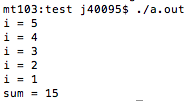
\includegraphics[clip, width=6.5cm]{kadai1-gcc.png}
          \hspace{3.0cm} gccにおけるコンパイル結果
        \end{center}
      \end{minipage}

      % 2
      \begin{minipage}{0.5\hsize}
        \begin{center}
          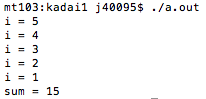
\includegraphics[clip, width=6.5cm]{kadai1-xcc.png}
          \hspace{3.0cm} 本課題によるコンパイル結果
        \end{center}
      \end{minipage}

    \end{tabular}
    \caption{実行結果}
  \end{center}
\end{figure}

\section{評価}
本課題のすべての拡張について変更を加え,例プログラムの結果も正しいものとなったので,課題を十分達成出来たと考える.

\section{考察}
本課題では,変数について大域変数のみの拡張であったため,codegen\_expression\_id内において条件分岐を用いて左辺値と右辺値を別に処理をしたが,
今後,ローカル変数やポインタを実装する際,すべての場合で条件分岐をすると煩雑になるため,右辺値用と左辺値用で関数を別で考えたほうが今後の拡張にむけて
展望があると感じた.\\
2項の小なり比較を行うsetl命令を調べている際に,2項のイコール比較を行うsete命令,2項の大なり比較を行うsetg命令についても知識を得られたので,今後の拡張のために記憶をしておきたいと思う.

\section{まとめ}
コードの理解に時間がかかったが,前期のコンパイラ構成の授業と合わせ,本課題によってコンパイラの動きをより理解できた.\\
MieruCompilerにより,どこのコードがどのアセンブリを生成しているのかが視覚的に分かりやすかったので課題をこなすにおいてとても助かったが,その分理解が後回しになってしまっていた
所があった.以降の課題については,まず自分の頭で考え,実行して正しく挙動しなかったときにMieruCompilerを使用したいと思う.
\end{document}
